\documentclass[]{beamer}
%\usepackage[MeX]{polski}
%\usepackage[cp1250]{inputenc}
\usepackage{polski}
\usepackage[utf8]{inputenc}
\beamersetaveragebackground{blue!10}
\usetheme{Warsaw}
\usecolortheme[rgb={0.1,0.5,0.7}]{structure}
\usepackage{beamerthemesplit}
\usepackage{multirow}
\usepackage{multicol}
\usepackage{array}
\usepackage{graphicx}
\usepackage{enumerate}
\usepackage{amsmath} %pakiet matematyczny
\usepackage{amssymb} %pakiet dodatkowych symboli

\author{Jarema Rydzewski - Bączek}
\title{Lunar Reconnaissance Orbiter}
\date{}

\begin{document}
\frame
{
\maketitle
}
\frame
{
\frametitle{Krotki Opis}
Lunar Reconnaissance Orbiter (LRO) – amerykańska sonda kosmiczna. Sztuczny satelita Księżyca. Podstawowym zadaniem sondy jest przeprowadzanie obserwacji na potrzeby programu lotów załogowych na Księżyc.
\begin{center}
\begin{figure}
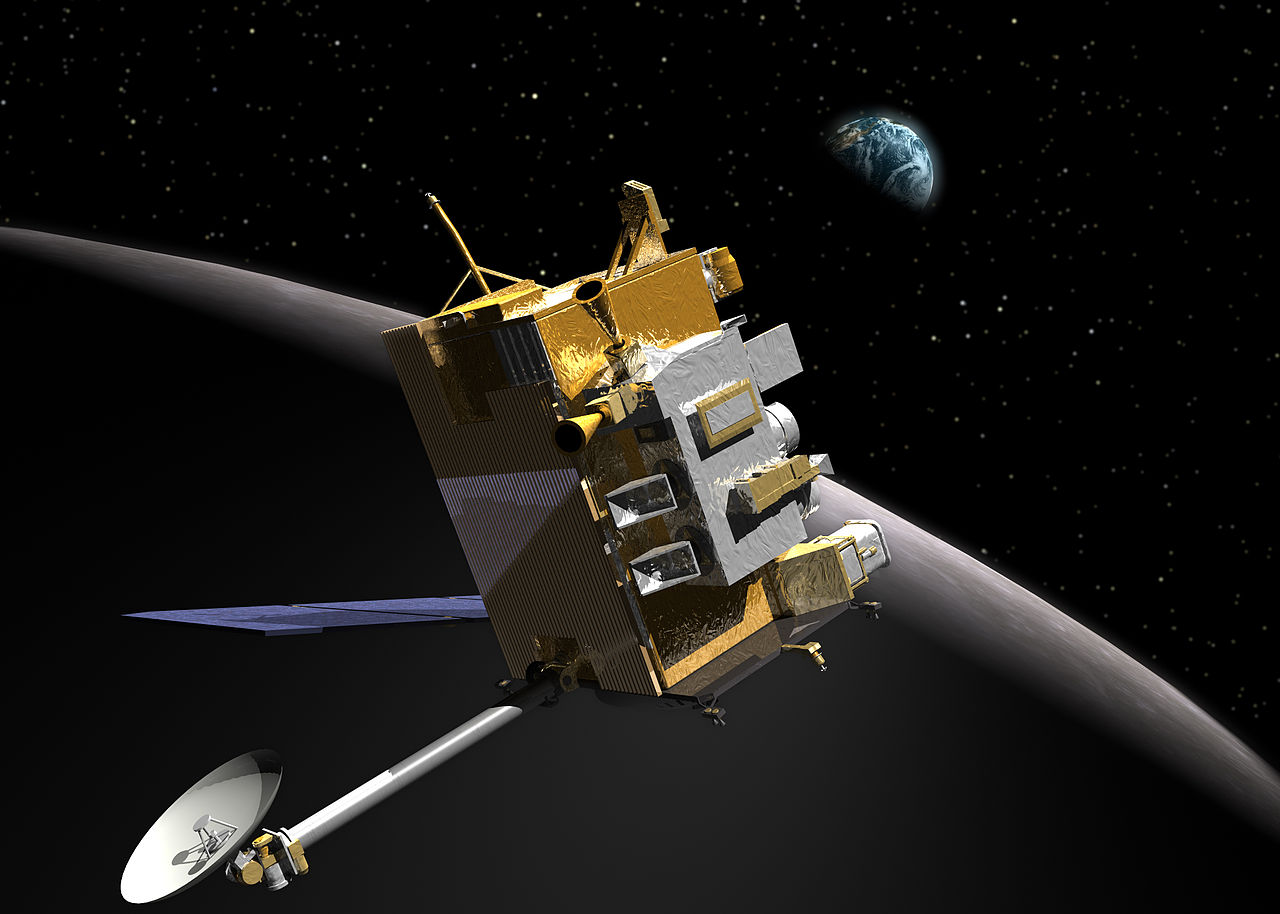
\includegraphics[scale=0.65]{sonda.jpg}
\end{figure}
\end{center}
}
\frame
{
\frametitle{Cele Misji}
\begin{itemize}
\item Wykonanie szczegółowych map topograficznych powierzchni Księżyca.
\item Obserwacja regionów biegunowych Księżyca, w tym obszarów wiecznie zacienionych.
\item Identyfikacja miejsc lądowań dla przyszłych załogowych i bezzałogowych misji księżycowych.
\item Pomiary poziomów promieniowania kosmicznego na orbicie wokółksiężycowej.
\item Identyfikacja złóż lodu wodnego i innych potencjalnych surowców możliwych do przyszłej eksploatacji.
\end{itemize}
}
\frame
{
\frametitle{Konstrukcja Sondy}
Sonda jest stabilizowana trójosiowo. Do boku statku przymocowane jest pojedyncze, złożone z trzech paneli, skrzydło ogniw słonecznych o powierzchni 10,7 m$^2$. Dostarcza ono energię o mocy 1850 W (pod koniec misji), dające średnio 800 W podczas każdej orbity. Ogniwa ładują baterie litowo-jonowe o pojemności 80 Ah. Maksymalna prędkość przesyłania danych na Ziemię (w paśmie Ka i paśmie S) wynosi 100 megabitów na sekundę. Dziennie przesyłane jest do 461 gigabitów danych. Całkowita masa startowa sondy wynosiła 1916 kg, w tym 898 kg paliwa dla silników korekcyjnych.

Sonda LRO została skonstruowana w należącym do NASA ośrodku Goddard Space Flight Center.
}
\frame
{
\frametitle{Instrumenty Naukowe}
Na pokładzie sondy znajduje się 6 podstawowych instrumentów naukowych oraz dodatkowy instrument eksperymentalny (Mini-RF).
\begin{itemize}
\item Cosmic Ray Telescope for the Effects of Radiation (CRaTER) 
\item Diviner Lunar Radiometer Experiment (DLRE) 
\item Lyman-Alpha Mapping Project (LAMP) 
\item Lunar Exploration Neutron Detector (LEND)
\item Lunar Orbiter Laser Altimeter (LOLA) 
\item Lunar Reconnaissance Orbiter Camera (LROC) — zestaw 3 kamer:
\item 2 kamery wąskokątne (NACs) 
\item kamera szerokokątna (WAC) 
\item Miniature Radio-Frequency Technology Demonstration (Mini-RF)
\end{itemize}
}
\frame
{
\frametitle{Przebieg Misji}
\begin{itemize}
\item 23 czerwca 2009 o 09:47 UTC
\item 24 czerwca 2009 o 10:56 UTC
\item 25 czerwca 2009 o 10:32 UTC
\item 26 czerwca 2009 12:25 UTC
\item 27 czerwca 2009
\item 30 czerwca 2009
\item 20 sierpnia 2009
\end{itemize}
}
\frame
{
\frametitle{Źródło}
https://pl.wikipedia.org/wiki/Lunar\_Reconnaissance\_Orbiter
}
\frame
{
\begin{center}
Dziękuje za Uwagę
\end{center} 
}
\end{document}
